% ----------------------------------------------------------
% CONFIGURAÇÂO DO DOCUMENTO
% ----------------------------------------------------------
\documentclass[
	% -- opções da classe memoir --
	12pt,				% tamanho da fonte
	openright,			% capítulos começam em pág ímpar (insere página vazia caso preciso)
	oneside,			% para impressão em verso e anverso. Oposto a oneside
	a4paper,			% tamanho do papel. 
	% -- opções da classe abntex2 --
	%chapter=TITLE,		% títulos de capítulos convertidos em letras maiúsculas
	%section=TITLE,		% títulos de seções convertidos em letras maiúsculas
	%subsection=TITLE,	% títulos de subseções convertidos em letras maiúsculas
	%subsubsection=TITLE,% títulos de subsubseções convertidos em letras maiúsculas
	% -- opções do pacote babel --
	english,			% idioma adicional para hifenização
	french,				% idioma adicional para hifenização
	spanish,			% idioma adicional para hifenização
	brazil				% o último idioma é o principal do documento
	]{abntex2}

% ---
% Pacotes básicos 
% ---
\usepackage{lmodern}			% Usa a fonte Latin Modern			
\usepackage[T1]{fontenc}		% Selecao de codigos de fonte.
\usepackage[utf8]{inputenc}		% Codificacao do documento (conversão automática dos acentos)
\usepackage{lastpage}			% Usado pela Ficha catalográfica
\usepackage{indentfirst}		% Indenta o primeiro parágrafo de cada seção.
\usepackage{color}				% Controle das cores
\usepackage{graphicx}			% Inclusão de gráficos
\usepackage{microtype} 			% para melhorias de justificação
% ---
		
% ---
% Pacotes adicionais, usados apenas no âmbito do Modelo Canônico do abnteX2
% ---
\usepackage{lipsum}				% para geração de dummy text
% ---

% ---
% Pacotes de citações
% ---
\usepackage[brazilian,hyperpageref]{backref}	 % Paginas com as citações na bibl
\usepackage[alf]{abntex2cite}	% Citações padrão ABNT

% --- 
% CONFIGURAÇÕES DE PACOTES
% --- 

% ---
% Configurações do pacote backref
% Usado sem a opção hyperpageref de backref
\renewcommand{\backrefpagesname}{Citado na(s) página(s):~}
% Texto padrão antes do número das páginas
\renewcommand{\backref}{}
% Define os textos da citação
\renewcommand*{\backrefalt}[4]{
	\ifcase #1 %
		Nenhuma citação no texto.%
	\or
		Citado na página #2.%
	\else
		Citado #1 vezes nas páginas #2.%
	\fi}%
% ---

% ----------------------------------------------------------
% ELEMENTOS DA CAPA
% ----------------------------------------------------------
% ---
% Informações de dados para CAPA e FOLHA DE ROSTO
% ---
\titulo{Definição de Perfis de Utilização e Predição de Problemas de Automóveis Baseados em Técnicas de Aprendizado de Máquina}
\autor{Cephas Alves da Silveira Barreto}
\local{Brasil}
\data{2017, v1.0}
\orientador{Prof. Dr. João Carlos Xavier Júnior}
\coorientador{Prof. Dr. Ivanovitch Medeiros Dantas da Silva}
\instituicao{%
  Universidade Federal do Rio Grande do Norte -- UFRN
  \par
  Instituto Metrópole Digital -- IMD
  \par
  Programa de Pós-Graduação em Engenharia de Software -- PPgSW}
\tipotrabalho{Dissertação (Mestrado)}
% O preambulo deve conter o tipo do trabalho, o objetivo, 
% o nome da instituição e a área de concentração 
\preambulo{Dissertação de Mestrado  apresentada ao Programa de Pós-graduação em Engenharia de Software da Universidade Federal do Rio Grande do Norte como requisito parcial para a obtenção do grau de Mestre em Engenharia de Software.}
% ---

% ----------------------------------------------------------
% APARENCIA DO PDF FINAL 
% ----------------------------------------------------------
% Configurações de aparência do PDF final

% alterando o aspecto da cor azul
\definecolor{blue}{RGB}{41,5,195}

% informações do PDF
\makeatletter
\hypersetup{
     	%pagebackref=true,
		pdftitle={\@title}, 
		pdfauthor={\@author},
    	pdfsubject={\imprimirpreambulo},
	    pdfcreator={LaTeX with abnTeX2},
		pdfkeywords={abnt}{latex}{abntex}{abntex2}{trabalho acadêmico}, 
		colorlinks=true,       		% false: boxed links; true: colored links
    	linkcolor=blue,          	% color of internal links
    	citecolor=blue,        		% color of links to bibliography
    	filecolor=magenta,      		% color of file links
		urlcolor=blue,
		bookmarksdepth=4
}
\makeatother
% --- 

% --- 
% Adicionado para evitar warning de Uppercase
% --- 
\pdfstringdefDisableCommands{\let\uppercase\relax}

% --- 
% Espaçamentos entre linhas e parágrafos 
% --- 

% O tamanho do parágrafo é dado por:
\setlength{\parindent}{1.3cm}

% Controle do espaçamento entre um parágrafo e outro:
\setlength{\parskip}{0.2cm}  % tente também \onelineskip

% ---
% compila o indice
% ---
\makeindex
% ---


% ----------------------------------------------------------
% ----------------------------------------------------------
% Início do documento
% ----------------------------------------------------------
% ----------------------------------------------------------
\begin{document}

% Seleciona o idioma do documento (conforme pacotes do babel)
\selectlanguage{brazil}
% Retira espaço extra obsoleto entre as frases.
\frenchspacing 

% ----------------------------------------------------------
% ELEMENTOS PRÉ-TEXTUAIS
% ----------------------------------------------------------
% \pretextual

% ----------------------------------------------------------
% CAPA
% ----------------------------------------------------------
% Mude para usar capa limpa ou customizada (Includes/Capa.tex)
\imprimircapa

% ----------------------------------------------------------
% FOLHA DE ROSTO
% ----------------------------------------------------------
% Folha de rosto (o * indica que haverá a ficha bibliográfica)
\imprimirfolhaderosto*

% ----------------------------------------------------------
% FICHA BIBLIOGRAFICA
% ----------------------------------------------------------
% ---
% Inserir a ficha bibliografica
% ---

% Isto é um exemplo de Ficha Catalográfica, ou ``Dados internacionais de
% catalogação-na-publicação''. Você pode utilizar este modelo como referência. 
% Porém, provavelmente a biblioteca da sua universidade lhe fornecerá um PDF
% com a ficha catalográfica definitiva após a defesa do trabalho. Quando estiver
% com o documento, salve-o como PDF no diretório do seu projeto e substitua todo
% o conteúdo de implementação deste arquivo pelo comando abaixo:
%
% \begin{fichacatalografica}
%     \includepdf{fig_ficha_catalografica.pdf}
% \end{fichacatalografica}

\begin{fichacatalografica}
	\sffamily
	\vspace*{\fill}					% Posição vertical
	\begin{center}					% Minipage Centralizado
	\fbox{\begin{minipage}[c][8cm]{13.5cm}		% Largura
	\small
	\imprimirautor
	%Sobrenome, Nome do autor
	
	\hspace{0.5cm} \imprimirtitulo  / \imprimirautor. --
	\imprimirlocal, \imprimirdata-
	
	\hspace{0.5cm} \pageref{LastPage} p. : il. (algumas color.) ; 30 cm.\\
	
	\hspace{0.5cm} \imprimirorientadorRotulo~\imprimirorientador\\
	
	\hspace{0.5cm}
	\parbox[t]{\textwidth}{\imprimirtipotrabalho~--~\imprimirinstituicao,
	\imprimirdata.}\\
	
	\hspace{0.5cm}
		1. Machine Learning. 
		2. Driving Behavior.
		I. XAVIER JÚNIOR, João Carlos.
        II. Universidade Federal Do Rio Grande do Norte.
        III. Instituto Metrópole Digital 
		IV. Definição de Perfis de Utilização e Predição de Problemas de Automóveis Baseados em Técnicas de Aprendizado de Máquina			
	\end{minipage}}
	\end{center}
\end{fichacatalografica}
% ---

% ----------------------------------------------------------
% ERRATA
% ----------------------------------------------------------
\begin{errata}
Elemento opcional da \citeonline[4.2.1.2]{NBR14724:2011}. Exemplo:

\vspace{\onelineskip}

FERRIGNO, C. R. A. \textbf{Tratamento de neoplasias ósseas apendiculares com
reimplantação de enxerto ósseo autólogo autoclavado associado ao plasma
rico em plaquetas}: estudo crítico na cirurgia de preservação de membro em
cães. 2011. 128 f. Tese (Livre-Docência) - Faculdade de Medicina Veterinária e
Zootecnia, Universidade de São Paulo, São Paulo, 2011.

\begin{table}[htb]
\center
\footnotesize
\begin{tabular}{|p{1.4cm}|p{1cm}|p{3cm}|p{3cm}|}
  \hline
   \textbf{Folha} & \textbf{Linha}  & \textbf{Onde se lê}  & \textbf{Leia-se}  \\
    \hline
    1 & 10 & auto-conclavo & autoconclavo\\
   \hline
\end{tabular}
\end{table}

\end{errata}
% ---

% ----------------------------------------------------------
% FOLHA DE APROVACAO
% ----------------------------------------------------------
% Folha de aprovação
\begin{folhadeaprovacao}
	%\setlength{\ABNTsignthickness}{0.4pt}
	%\setlength{\ABNTsignwidth}{10cm}
	
	% Informações gerais acerca do trabalho 
	% (nome do autor, título, instituição à qual é submetido e natureza)
	\noindent 
	Dissertação de Mestrado sob o título \textit{Definição de Perfis de Utilização e Predição de Problemas de Automóveis Baseados em Técnicas de Aprendizado de Máquina} apresentada por \textbf{Cephas Alves da Silveira Barreto} e aceita pelo Programa de Pós-graduação em Engenharia de Software da Universidade Federal do Rio Grande do Norte, sendo aprovada por todos os membros da banca examinadora abaixo especificada:
		
	% Membros da banca examinadora e respectivas filiações
	\assinatura
	{
		Prof. Dr. Fulano de tal,PhD   			                  \\
		{\small Presidente}											          \smallskip\\ 
		{\footnotesize
			IMD -- Instituto Metrópole Digital		   \\
		  	UFRN -- Universidade Federal do Rio Grande do Norte
		}
   }
      
   \assinatura
	{
      Nome completo do examinador e titulação   			                  \\
		{\small Examinador}											          \smallskip\\ 
		{\footnotesize
			Departamento		\\
		  	Universidade
		}
   }   
   
   \assinatura
	{
      Nome completo do examinador e titulação   			                  \\
		{\small Examinador}											          \smallskip\\ 
		{\footnotesize
			Departamento		\\
		  	Universidade
		}
	}
		
	\vfill
	
	\begin{center}
		Natal-RN, data da defesa (dia, mês e ano).
	\end{center}
\end{folhadeaprovacao}


\begin{folhadeaprovacao}

  \begin{center}
    {\ABNTEXchapterfont\large\imprimirautor}

    \vspace*{\fill}\vspace*{\fill}
    \begin{center}
      \ABNTEXchapterfont\bfseries\Large\imprimirtitulo
    \end{center}
    \vspace*{\fill}
    
    \hspace{.45\textwidth}
    \begin{minipage}{.5\textwidth}
        \imprimirpreambulo
    \end{minipage}%
    \vspace*{\fill}
   \end{center}
        
   Trabalho aprovado. \imprimirlocal, 24 de novembro de 2012:

   \assinatura{\textbf{\imprimirorientador} \\ Orientador} 
   \assinatura{\textbf{Professor} \\ Convidado 1}
   \assinatura{\textbf{Professor} \\ Convidado 2}
   %\assinatura{\textbf{Professor} \\ Convidado 3}
   %\assinatura{\textbf{Professor} \\ Convidado 4}
      
   \begin{center}
    \vspace*{0.5cm}
    {\large\imprimirlocal}
    \par
    {\large\imprimirdata}
    \vspace*{1cm}
  \end{center}
  
\end{folhadeaprovacao}


% ----------------------------------------------------------
% DEDICATORIA
% ----------------------------------------------------------
% Dedicatória

\chapter*{}
\vspace{15cm}
\begin{flushright}
	Homenagem que o autor presta a uma ou mais pessoas.
\end{flushright}


% ----------------------------------------------------------
% AGRADECIMENTOS
% ----------------------------------------------------------
\input{Includes/Agradecimentos.tex}

% ----------------------------------------------------------
% EPIGRAFE
% ----------------------------------------------------------
\input{Includes/Epigrafe.tex}

% ----------------------------------------------------------
% RESUMO
% ----------------------------------------------------------
\chapter*{}
% Resumo em língua vernácula
\begin{center}
	{\Large{\textbf{Definição de Perfis de Utilização e Predição de Problemas de Automóveis Baseados em Técnicas de Aprendizado de Máquina
}}}
\end{center}

\vspace{1cm}

\begin{flushright}
	Autor: Cephas Alves da Silveira Barreto\\
	Orientador: Prof. Dr. João Carlos Xavier Júnior
\end{flushright}

\vspace{1cm}

\begin{center}
	\Large{\textsc{\textbf{Resumo}}}
\end{center}

\noindent Considerando o incremento no número de automóveis nos grandes centros urbanos e os problemas que decorrem desse contexto, possuir ferramentas capazes de extrair informações a respeito do comportamento dos motoristas, torna-se uma importante estratégia para a diminuição dos problemas já existentes e também para a prevenção de problemas que possam vir a ocorrer neste domínio, como acidentes de trânsito, aumento da poluição, congestionamentos, distribuição dos tipos de transportes no espaço urbano e etc. Este artigo apresenta um estudo sobre as estratégias de definição de perfis de motoristas, mais especificamente as estratégias que utilizam técnicas de Aprendizado de Máquina para esse fim, propõe uma comparação entre diversas abordagens utilizadas para a definição de perfis de motoristas, enfatizando seus pontos fortes e também analisando possíveis limitações existentes.

\noindent\textit{Palavras-chave}: Machine Learning. Driving Behavior.




% resumo em inglês
%\begin{resumo}[Abstract]
% \begin{otherlanguage*}{english}
%   This is the english abstract.

%   \vspace{\onelineskip}
 
%   \noindent 
%   \textbf{Keywords}: latex. abntex. text editoration.
% \end{otherlanguage*}
%\end{resumo}


% ----------------------------------------------------------
% LISTA DE ILUSTRACOES
% ----------------------------------------------------------
\chapter*{}
% ---
% inserir lista de ilustrações
% ---
\pdfbookmark[0]{\listfigurename}{lof}
\listoffigures*
\cleardoublepage
% ---

% ----------------------------------------------------------
% LISTA DE TABELAS
% ----------------------------------------------------------
% ---
% inserir lista de tabelas
% ---
\pdfbookmark[0]{\listtablename}{lot}
\listoftables*
\cleardoublepage
% ---

% ----------------------------------------------------------
% LISTA DE ABREVIATURAS E SIGLAS
% ----------------------------------------------------------
% ---
% inserir lista de abreviaturas e siglas
% ---
\begin{siglas}
  \item[ABNT] Associação Brasileira de Normas Técnicas
  \item[abnTeX] ABsurdas Normas para TeX
\end{siglas}
% ---

% ----------------------------------------------------------
% LISTA DE SIMBOLOS
% ----------------------------------------------------------
\input{Includes/ListaSimbolos.tex}

% ----------------------------------------------------------
% SUMARIO
% ----------------------------------------------------------
% ---
% inserir o sumario
% ---
\pdfbookmark[0]{\contentsname}{toc}
\tableofcontents*
\cleardoublepage
% ---


% ----------------------------------------------------------
% ----------------------------------------------------------
% ELEMENTOS TEXTUAIS
% ----------------------------------------------------------
% ----------------------------------------------------------
\textual

% ----------------------------------------------------------
% Introdução
% ----------------------------------------------------------
% Introdução
\chapter*{Introdução}

Segundo a Organização das Nações Unidas \cite{un2010state}, em 2050, 91,4\% da população da América Latina viverá em áreas urbanas. Assim como em outros países, se agravam no Brasil os problemas decorrentes do aumento da densidade demográfica nos centros urbanos. Poluição, epidemias, congestionamentos, violência e outros problemas têm se tornado uma questão urgente para os gestores dos espaços urbanos.  A poluição atmosférica, por exemplo, agravada com o aumento do número de veículos, é responsável por cerca de 20 mil óbitos por ano no Brasil \cite{arbex2012poluiccao}. O aumento do número de veículos é outro problema que vem tomando grandes proporções nas grandes cidades. Como pode ser visto na Figura \ref{fig:crescimentoveiculos}, esse problema tem se agravado especialmente a partir do ano de 2001 \cite{INCT2013evoluccao}.

\begin{figure}[ht]
\centering
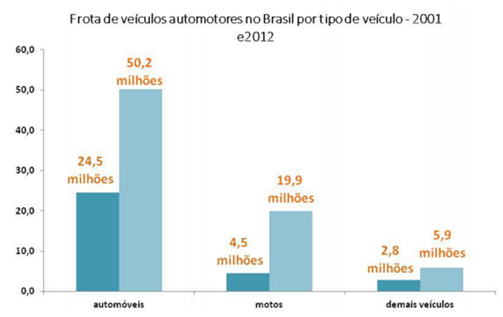
\includegraphics[width=4.5in]{Imagens/carrosUp.png}. 
\caption{Crescimento de veículos no Brasil}
\label{fig:crescimentoveiculos}
\end{figure}

Nesse período, por exemplo, o crescimento do número de veículos nas regiões metropolitanas brasileiras foi de no mínimo 73,1\% (valor alcançado pelo Rio de Janeiro), e mais que dobrou em casos como Curitiba, Belém e outras, como é possível observar na Figura \ref{fig:crescimentocarros}. Isso indica que o crescimento do número de veículos está acontecendo com valores relativamente altos, e que é necessário ter formas de oferecer respaldo para as iniciativas que tentem lidar com o grande número de veículos e problemas decorrentes.

\begin{figure}[ht]
\centering
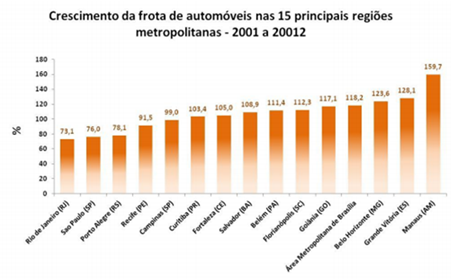
\includegraphics[width=4.5in]{Imagens/carrosUpBrasil.png}.  
\caption{Crescimento de carros nas regiões metropolitanas}
\label{fig:crescimentocarros}
\end{figure}

Ainda nas grandes regiões metropolitanas é possível observar que, em grande parte dos casos, o desenvolvimento urbano não acontece de forma sustentável \cite{rolnik2011crescimento} e não consegue acompanhar demandas urgentes como a necessidade de transporte para pessoas que vive nas metrópoles. Esse fato, aliado ao crescente número de pessoas, acaba transformando o ambiente urbano num plano ideal para o agravamento mais acelerado dos problemas locais. Parte desses problemas se relaciona de forma estreita com os veículos utilizados diariamente pelas pessoas.

Segundo a Wharton School (2013)\cite{WHARTON2013}, cerca de 6 a 7 bilhões de reais de prejuízo foram causados em todo o Brasil, apenas pelos acidentes envolvendo veículos no ano de 2013. Tais prejuízos financeiros se somam a tantos outros problemas, como por exemplo: os ambientais, devido à grande quantidade de poluentes lançados no ambiente; transtornos psicológicos nas pessoas envolvidas em acidentes com veículos; na produtividade, devido à grande quantidade de tempo desperdiçado com problemas de infraestrutura, trânsito ou nos próprios veículos, e etc. Com isso fica claro que o acúmulo de veículos traz consigo uma grande quantidade de problemas, dessa forma é importante pensar em abordagens que possam reduzir ou eliminar tais problemas.

Motivados pelos problemas relacionados acima e com o objetivo de oferecer uma forma de auxiliar no melhor uso de veículos, alguns trabalhos recentes \cite{zhang2016driver,amsalu2016driver,meseguer2015assessing,eren2012estimating}, têm focado em abordagens que permitem a criação de perfis automáticos de usuários (motoristas) de automóveis. Os resultados desses trabalhos possibilitam entender como um motorista utiliza o seu veículo, o que pode trazer benefícios relacionados à eficiência energética, infraestrutura das cidades, seguridade automotiva, planejamento urbano e etc. Neste artigo será abordado o atual estado do uso de técnicas de Aprendizado de Máquina (AM) para a definição de perfis de utilização de veículos e também, proposta uma abordagem para essa forma de descoberta de perfis de motoristas.

O restante deste artigo está organizado da seguinte forma. Em seguida, a Seção XXXXX aborda os trabalhos relacionados à descoberta de perfis de utilização de automóveis, mostrando os aspectos gerais e também aspectos mais específicos dos principais artigos. A Seção XXXXX propõe uma abordagem de solução do problema em questão e faz uma breve contextualização de suas características com o que foi abordado na seção XXXXXX. Por fim, a Seção XXXXX aborda os resultados que se quer atingir com a abordagem proposta.

\section{Organização do trabalho}

Nesta seção deve ser apresentado como está organizado o trabalho, sendo descrito, portanto, do que trata cada capítulo.
%\chapter*{Introdução}
%\addcontentsline{toc}{chapter}{Introdução}


% ----------------------------------------------------------
% PARTE
% ----------------------------------------------------------
\part{Preparação da pesquisa}


% ----------------------------------------------------------
% Finaliza a parte no bookmark do PDF
% para que se inicie o bookmark na raiz
% e adiciona espaço de parte no Sumário
% ----------------------------------------------------------
\phantompart

% ----------------------------------------------------------
% CONCLUSAO
% ----------------------------------------------------------
\chapter{Conclusão}

% ----------------------------------------------------------
% ----------------------------------------------------------
% ELEMENTOS PÓS-TEXTUAIS
% ----------------------------------------------------------
% ----------------------------------------------------------
\postextual

% ----------------------------------------------------------
% Referências bibliográficas
% ----------------------------------------------------------
\bibliography{abntex2-modelo-references}

% ----------------------------------------------------------
% Glossário
% ----------------------------------------------------------
%\glossary

% ----------------------------------------------------------
% Apêndices
% ----------------------------------------------------------
% ---
% Inicia os apêndices
% ---
\begin{apendicesenv}

% Imprime uma página indicando o início dos apêndices
\partapendices
% ----------------------------------------------------------
\chapter{Quisque libero justo}
% ----------------------------------------------------------

\lipsum[50]

% ----------------------------------------------------------
\chapter{Nullam elementum urna vel imperdiet sodales elit ipsum pharetra ligula
ac pretium ante justo a nulla curabitur tristique arcu eu metus}
% ----------------------------------------------------------
\lipsum[55-57]

\end{apendicesenv}

% ----------------------------------------------------------
% Anexos
% ----------------------------------------------------------
\begin{anexosenv}
% Imprime uma página indicando o início dos anexos
\partanexos
% ---
\chapter{Morbi ultrices rutrum lorem.}
% ---
\lipsum[30]
% ---
\chapter{Cras non urna sed feugiat cum sociis natoque penatibus et magnis dis
parturient montes nascetur ridiculus mus}
% ---
\lipsum[31]

% ---
\chapter{Fusce facilisis lacinia dui}
% ---
\lipsum[32]
\end{anexosenv}



%---------------------------------------------------------------------
% INDICE REMISSIVO
%---------------------------------------------------------------------

\phantompart
\printindex
%---------------------------------------------------------------------

\end{document}
